% =========================================================================== %
% Yes. This is a document.

\documentclass[
	ngerman,
	aspectratio=169,
	table
]{beamer}

% =========================================================================== %
% Theme
\usepackage{scrlfile}
	\ReplacePackage{beamerthemeSHUR}{./sty/beamerthemeSHUR}
	\ReplacePackage{beamerinnerthemefancy}{./sty/beamerinnerthemefancy}
	\ReplacePackage{beamerouterthemedecolines}{./sty/beamerouterthemedecolines}
	\ReplacePackage{beamercolorthemechameleon}{./sty/beamercolorthemechameleon}

\usetheme[
	pageofpages=von,
	bullet=circle,
	titleline=true,
	alternativetitlepage=true,
	watermark="",
	watermarkheight=0px,
	watermarkheightmult=0
	]
{SHUR}

% =========================================================================== %
% the usual stuff

\usepackage[utf8]{inputenc}
\usepackage[T1]{fontenc}
\usepackage{babel}
\usepackage{lmodern}
\usepackage{microtype}
\usepackage{csquotes}

\usepackage{tabularx}
\usepackage{booktabs}
\usepackage{multirow}

\usepackage{color, colortbl}
\usepackage{xcolor}
	\definecolor{tabhighlight}{RGB}{230,240,255}

\usepackage{tabto}

\usepackage{minted}
	\usemintedstyle{friendly}

\usepackage{tikz}
	\usetikzlibrary{positioning}
	\usetikzlibrary{matrix}
	\usetikzlibrary{shapes.geometric}
	\usetikzlibrary{backgrounds}
	\usetikzlibrary{calc}
	\usetikzlibrary{decorations.pathreplacing}
	\tikzstyle{every picture}+=[remember picture] 
\usepackage{adjustbox}

\usepackage[most]{tcolorbox}
	\tcbsetforeverylayer
		{colback=cyan!10!white,
		 colframe=cyan!75!black,
		 arc=0pt,
		 outer arc=0pt
		}
	\newtcolorbox{codebox}[1][Code]
		{colback=black!5!white,
		 colframe=blue!40!black,
		 title=#1,
		 leftupper=6mm
		}
	\newtcolorbox{cmdbox}[1][Kommandozeilen-Befehl]
		{colback=black,
		 coltext=white,
		 fontupper=\ttfamily ,
		 colframe=blue!40!black,
		 title=#1,
		 outer arc=0pt
		}
	\newtcolorbox{warnbox}[1][Beachte]
		{colback=black!5!white,
		 colframe=red!40!black,
		 title=#1
		}
	\newtcolorbox{hintbox}[1][Tipp]
		{colback=black!5!white,
		 colframe=green!40!black,
		 title=#1
		}
	\newenvironment{itembox}
		{\begin{tcolorbox}\begin{itemize}}%
		{\end{itemize}\end{tcolorbox}}
	\newtcolorbox{doublebox}[1][.3]
		{righthand width=#1\linewidth,
		 sidebyside,
		 sidebyside gap=6mm,
		 sidebyside align=center,
		 lower separated=false}
	
%==============================================================================%
% GLOBAL MACROS

\newcommand*{\zB}{z.\,B. }
\newcommand*{\ua}{u.\,a. }
\newcommand*{\ie}{d.\,h. }			%% dh is already a defined macro. Couldn't find out what it does.
\newcommand*{\idR}{i.\,d.\,R. }

\newcommand{\Thus}{\ensuremath{\Rightarrow}}
\newcommand{\thus}{\ensuremath{\rightarrow}}

\newcommand*{\tabcrlf}{\\ \midrule}			% actually still allows for optional argument

\newcommand*{\inPy}[1]{\mintinline{python}{#1}}

% =========================================================================== %

\author{Stefan Hartinger}
\title{Programmieren in Python}
\subtitle{Kursteil 1: Arbeitsumgebung und erste Schritte}
\institute{Universität Regensburg, Fakultät Physik}
\date{Wintersemester 2020/21}

% =========================================================================== %

\begin{document}
% =========================================================================== %

\begin{frame}[t,plain]
\titlepage
\end{frame}

% =========================================================================== %

\begin{frame}
%
\begin{center}

\includegraphics[width=.5\linewidth]{./gfx/intro}
\end{center}
%
\end{frame}

% =========================================================================== %

\begin{frame}{Unser Mantra}
%
\begin{center}
\begin{Huge}
\emph{Computer sind strunzdumm.}
\end{Huge}
\vspace{20pt}

Wir als Menschen erschließen uns implizit eine Menge an Informationen, und bewältigen dadurch unseren Alltag. Ein Computer kann das nicht. Wann immer auch nur der Hauch von Uneindeutigkeit besteht, wird der Computer den Dienst verweigern. Wann immer etwas automatisch geschieht, hat ein(e) ProgrammiererIn diesen automatismus bewusst eingebaut.
\vspace{10pt}

In diesem Kurs werden wir vor allem lernen, unser eigenes Denken zu analysieren und diese Ergebnisse dann in Code formulieren.
\end{center}
%
\end{frame}

% =========================================================================== %

\begin{frame}{Programmieren in Python -- Historisches Bla Bla}
%
\begin{itemize}
\item Seit 2003 durchgehend eine der Top 10 Sprachen im TIBOE-Index (basiert auf Web-Aktivität zu den verschiedenen Sprachen)
\item Erste Veröffentlichung 1991, kontinuierlich Weiterentwickelt
\item Aktueller \emph{Stable Release}: 3.8 (Inhalt des Kurses)
\item Major Versions nicht 100\% Kompatibel, Logik aber gleichbleibend und auf viele andere Sprachen übertragbar
\item \enquote{Batteries included} -- viele vorgefertigte Standard-Lösungen
\item Script-Sprache -- optimiert auf schnelle Entwicklung, gute Lesbarkeit und Portierbarkeit
\item Dafür oft langsamer in der Ausführung
\end{itemize}
%
\end{frame}

% =========================================================================== %

\begin{frame}{Grundbegriffe: Interpreter}
%
\begin{minipage}{.49\linewidth}
\begin{itemize}
\item Code: (mehr oder minder) menschliche Sprache
\item Computer: Numerierte Befehle, sehr kleinschrittig
\item Interpreter: Programm, das Code in Maschinensprache übersetzt
\item Interpreter tut dies \enquote{in Echtzeit}, Compiler bereiten vor
\item Vorteil: Interpreter kümmert sich um Maschinen-Spezifische Details; selber Code funktioniert auf (fast) allen Maschinen
\end{itemize}
\end{minipage}
%
%
\begin{minipage}[t]{.49\linewidth}
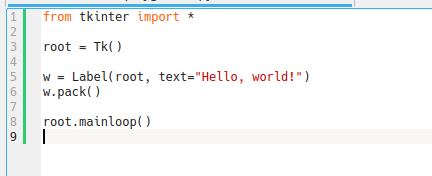
\includegraphics[width=\linewidth]{./gfx/TK-HelloWorld-Code}
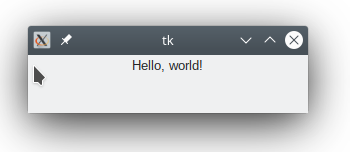
\includegraphics[width=\linewidth]{./gfx/TK-HelloWorld-Run}
\end{minipage}
%
\end{frame}

% =========================================================================== %

\begin{frame}
%
\begin{columns}[T]
\column{.5\linewidth}
\begin{Large}
{Grundbegriffe: Terminal}
\end{Large}
\begin{itemize}
\item Interpreter-Aufruf (wenigstens mittelbar) über ein \emph{Terminal}
\item Mensch-Maschine-Interface
\item Befehle in menschlicher (oder Menschen-ähnlicher) Sprache
\item Bis heute das \emph{Backend}, über das Computer funktionieren.
\item \emph{IDEs} (integrated development environment): mehr Komfort, aber uneinheitlich
\item Letztlich überall Terminal-Kenntnisse nötig, wo Programmiert werden soll
\end{itemize}
%
\column{.5\linewidth}
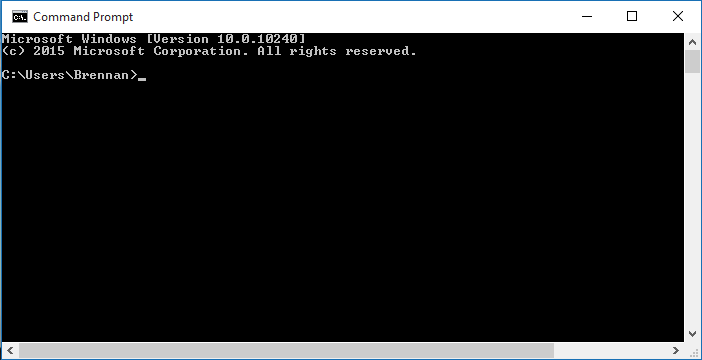
\includegraphics[width=\linewidth]{./gfx/cmd}
{\tiny Windows-Konsole: \texttt{cmd}}
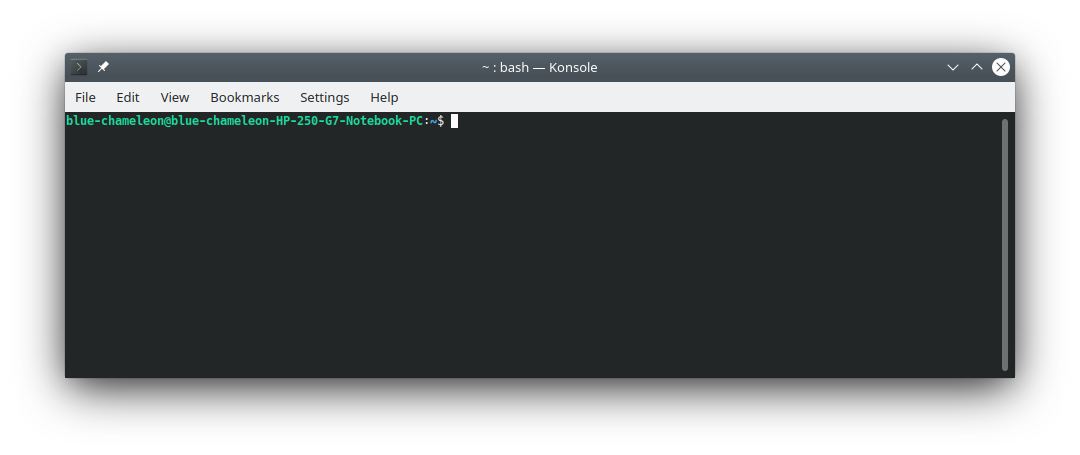
\includegraphics[width=\linewidth]{./gfx/bash}
{\tiny Linux-Konsole: \texttt{bash}}
\end{columns}
%
\end{frame}

% =========================================================================== %

\begin{frame}{Grundbegriffe: Arbeitsverzeichnis}
%
\begin{itemize}
\item Alle Dateien auf Computern: In Ordnern strukturiert
\item Mehrere Dateien mit gleichem Namen in verschiedenen Ordnern möglich
\item Computer muss wissen, welche Datei gemeint ist
\item Idee: Arbeitsverzeichnis: \emph{Wo bin ich gerade}
\end{itemize}
%
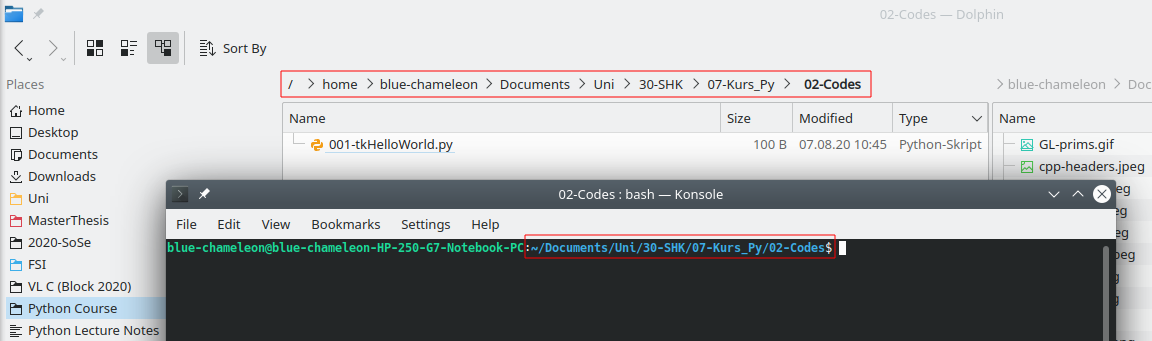
\includegraphics[width=\linewidth]{./gfx/paths}
%
\end{frame}

% =========================================================================== %

\begin{frame}{Programme Starten und Arbeitsverzeichnisse}
%
\begin{itemize}
\item In das richtige Verzeichnis wechseln: \texttt{cd}
	\begin{minipage}{\linewidth}
		\begin{minipage}{.49\linewidth}
		\begin{itemize}
		\item In einem Schritt mehrere Ebenen:\\
			\texttt{cd directory/subdirectory}
		\end{itemize}
		\end{minipage}
		%
		\begin{minipage}{.49\linewidth}
		\begin{itemize}
		\item Oder in mehreren Schritten:\\
			\texttt{cd directory}\\
			\texttt{cd subdirectory}
		\end{itemize}
		\end{minipage}
	\end{minipage}
	\item Eine Ebene zurück: zwei Punkte:\\
		\texttt{cd ..}
	\item Leerzeichen im Pfad? \Thus ~ mit Anführungszeichen einrahmen:\\
		\texttt{cd "Path with whitespaces"}
%	\end{itemize}
\item Name des Programms benennen -- läuft
\end{itemize}
%
%\includegraphics[width=\linewidth]{./gfx/RunRunnot}
%
\end{frame}

% =========================================================================== %

\begin{frame}{Parameter}
%
\begin{itemize}
\item Programme brauchen manchmal zusätzliche Informationen
\item Text hinter dem eigentlichen Befehl
\item Beispiel \texttt{cd}: Unterordner oder \texttt{..}
\item Durch Leerzeichen abgetrennt
\item Auch mehrere Parameter möglich, dann auch jeweils durch Leerzeichen getrennt
\item Problem: Dateinamen mit Leerzeichen
\item Lösung: \texttt{"Text mit Leerzeichen in Anführungszeichen"}
\item Beispiel
	\begin{itemize}
	\item \texttt{notepad ''some file I want to open.txt"}
	\end{itemize}
\end{itemize}
%
\end{frame}

% =========================================================================== %

\begin{frame}{Grundbegriffe: (Dateinamen-)Erweiterung oder Dateiendung}
%
\begin{itemize}
\item Konzept zur Unterscheidung von Datentypen
\item Namenschema \texttt{Inhalt.Typ}
\item Üblicherweise 1-3 Zeichen, seit den späten 90ern aber prinzipiell keine Grenzen
\item txt, pdf, docx, odt, ...
\item Unter Windows häufig ausgeblendet
\item Executables in Windows: \texttt{*.exe}
\item Unixoide Systeme (Linux, Mac OS): meist keine Erweiterungen
\item Python-Codes sollten aber in allen Betriebssystemen auf \texttt{*.py} enden
\end{itemize}
%
\end{frame}

% =========================================================================== %

\begin{frame}{\enquote{globale} Befehle}
%
\begin{itemize}
\item Soweit verstanden: Zum Ausführen muss Arbeitsverzeichnis gleich Speicherort des Programms sein.
\item Programme können Parameter verarbeiten und sogar brauchen
\item Wieso funktioniert dann \texttt{notepad ''some file I want to open.txt"}?
\item[\Thus] \enquote{Standard-Suchpfade}
\item[\Thus] In der Übung: Rechner so einrichten, dass \texttt{python myCode.py} oder \texttt{python3 myCode.py} funktioniert.
\item Funktioniert \idR automatisch bei der Installation
\end{itemize}
%
\end{frame}

% =========================================================================== %

\begin{frame}{Übersicht: Befehle (Windows)}
\begin{itemize}
\item Terminal Starten
	\begin{itemize}
	\item über Startleiste: Suche nach \texttt{Kommandozeile} oder \texttt{Command Line}
	\item über Ausführen-Dialog: \texttt{[Windows-Taste]} + \texttt{[R]}, und dann \texttt{cmd} eingeben
	\end{itemize}
\item Arbeitsverzeichnis wechseln
	\begin{itemize}
	\item In Unterordner wechseln: \texttt{cd Unterordner}
	\item In Überordner wechseln: \texttt{cd ..}
	\end{itemize}
\item Unsere Codes ausführen:
	\begin{itemize}
	\item \texttt{python myCode.py}
	\end{itemize}
\item Verzeichnisinhalt anzeigen:
	\begin{itemize}
	\item \texttt{dir}
	\end{itemize}
\end{itemize}
\end{frame}

% =========================================================================== %

\begin{frame}{Übersicht: Befehle (Linux und Mac OS)}
\begin{itemize}
\item Terminal Starten
	\begin{itemize}
	\item Meistens: \texttt{[CTRL]} + \texttt{[ALT]} + \texttt{[T]}
	\item Ansonsten: Anwendungs-Menü der grafischen Oberfläche \thus ~Suche nach Terminal
	\item Häufig in Reiter \emph{Applications/Utilities} oder \emph{System}
	\end{itemize}
\item Arbeitsverzeichnis wechseln
	\begin{itemize}
	\item In Unterordner wechseln: \texttt{cd Unterordner}
	\item In Überordner wechseln: \texttt{cd ..}
	\end{itemize}
\item Programm starten:
	\begin{itemize}
	\item \texttt{python3 myCode.py}
	\end{itemize}
\item Verzeichnisinhalt anzeigen:
	\begin{itemize}
	\item \texttt{ls}
	\end{itemize}
\end{itemize}
\end{frame}

% =========================================================================== %

\begin{frame}{Mini-Programme direkt in der Konsole starten}
%
\begin{minipage}[t]{.39\linewidth}
\begin{itemize}
\item In Konsole: Befehl \texttt{python} (bzw. \texttt{python3}) startet den Interpreter
\item Gleiches Fenster, aber Computer \enquote{versteht} jetzt Python-Befehle (dafür aber keine Konsolen-Befehle mehr).
\item Beispiel: \inPy{1+2}: Wert berechnen und direkt auf dem Bildschirm ausgeben
\item Zeilen beginnen mit \texttt{>{}>{}>}
\item Beenden: \texttt{quit()}
\end{itemize}
\end{minipage}
%
%
\begin{minipage}[t]{.59\linewidth}
\vspace{0pt}
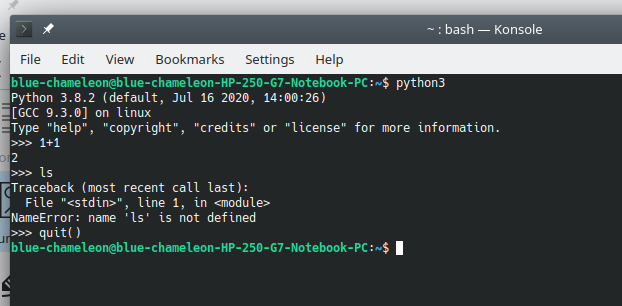
\includegraphics[width=\linewidth]{./gfx/interpreterConsole}
\end{minipage}
%
\end{frame}

% =========================================================================== %

\begin{frame}[fragile]{\enquote{echte Programme}: Über Scriptdatei}
%
\begin{minipage}[t]{.29\linewidth}
\vspace{0pt}
\begin{itemize}
\item Codes wachsen schnell auf mehrere Tausend Zeilen
\item Unpraktisch, das jedes mal neu eingeben zu müssen
\item[\Thus] Textdatei, in der alle Kommandos bereit stehen
\item Wird Zeile für Zeile abgearbeitet
\end{itemize}
\end{minipage}
%
%
\begin{minipage}[t]{.69\linewidth}
\vspace{0pt}
\begin{codebox}[Code: \texttt{001-helloWorld.py}]
\begin{minted}[linenos, fontsize=\scriptsize]{python}
print("Hello World")
\end{minted}
\end{codebox}
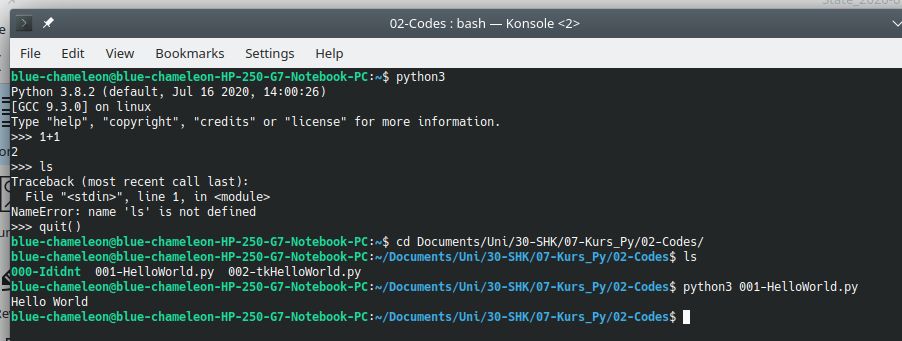
\includegraphics[width=\linewidth]{./gfx/print-HelloWorld-Run}
\end{minipage}
%
\end{frame}

% =========================================================================== %

\begin{frame}[fragile]{Die IDE \emph{Spyder}}
%
\begin{center}
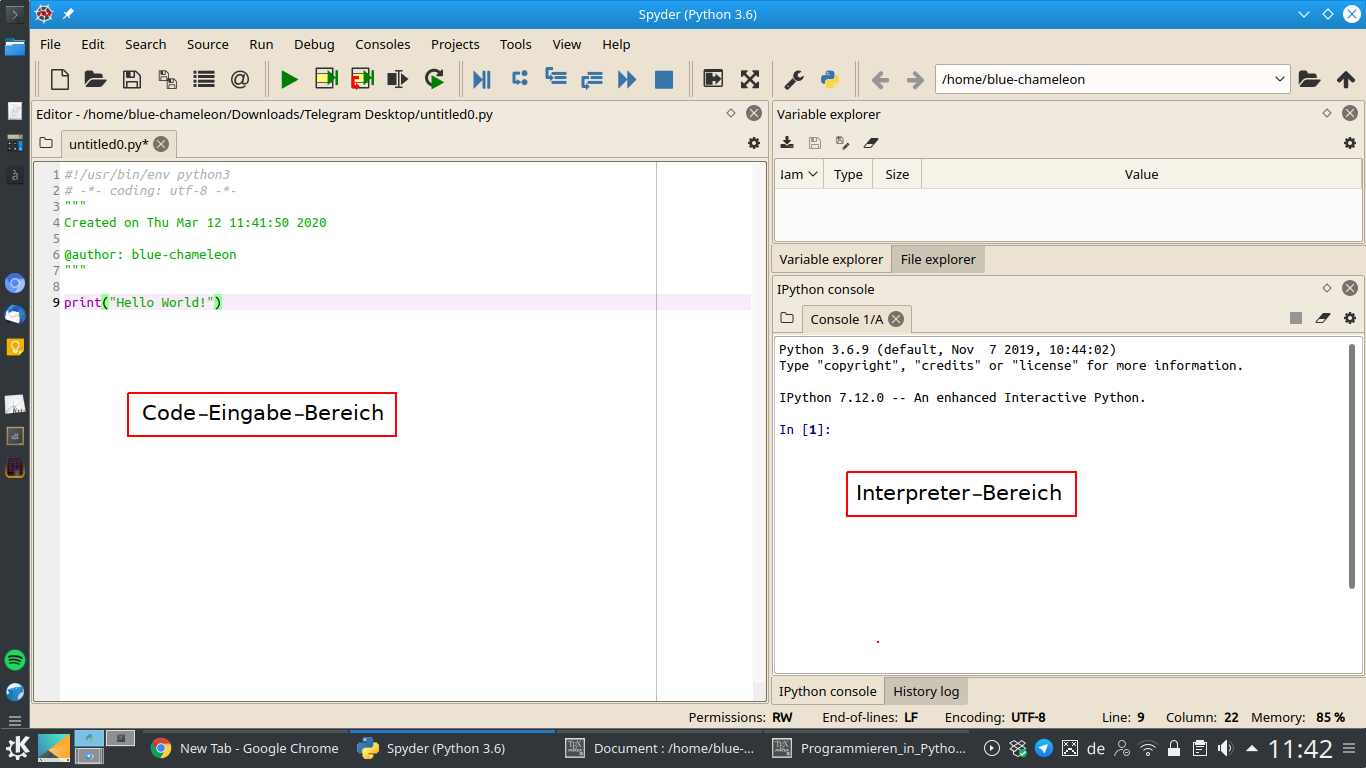
\includegraphics[width=.8\linewidth]{./gfx/Spyder}
\end{center}
%
\end{frame}

% =========================================================================== %

\begin{frame}[fragile]{Der Befehl \inPy{print}}
%
\begin{itemize}
\item Ausgabe von Text auf dem Bildschirm
\item Nötig für die Arbeit mit Script-Dateien
\item \emph{Parameter} in (runden Klammern)
\item Parameter: Texte, die Ausgegeben werden sollen, durch Kommata getrennt
\item Texte von \texttt{'}einfachen\texttt{'} oder \texttt{''}Doppelten\texttt{''} Anführungszeichen eingerahmt
\end{itemize}

\vspace{10pt}
\begin{minipage}{.49\linewidth}
\begin{codebox}[Code]
\begin{minted}[linenos, fontsize=\scriptsize]{python}
print("Text")
print("und noch", "mehr Text")
\end{minted}
\end{codebox}
%
\end{minipage}
\begin{minipage}{.49\linewidth}
\begin{cmdbox}[Ausgabe]
\begin{minted}[fontsize=\scriptsize]{text}
Text
und noch mehr Text
\end{minted}
\end{cmdbox}
\end{minipage}
\end{frame}

% =========================================================================== %

\begin{frame}{Fehlermeldungen}
%
\begin{minipage}[t]{.29\linewidth}
\begin{itemize}
\item Angabe des Fehlerorts (Datei, Zeile)
\item Bei Eingabe direkt in die Konsole: \texttt{<stdin>, line 1}
\item Kopie der Zeile, die nicht übersetzt werden konnte, z.\;T. mit Markierung was genau nicht stimmt
\end{itemize}
\end{minipage}
%
%
\begin{minipage}[t]{.69\linewidth}
\vspace{0pt}
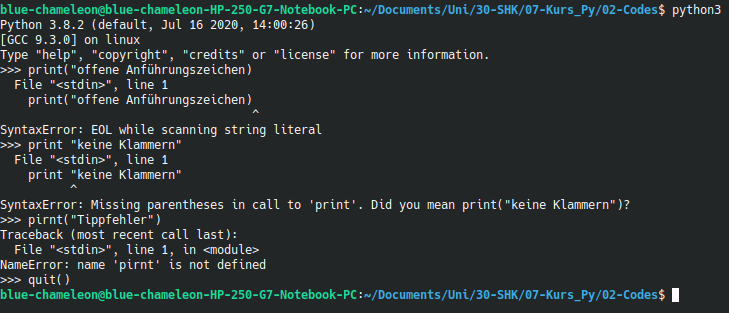
\includegraphics[width=\linewidth]{./gfx/errMsgs}
\end{minipage}
%
%
\begin{itemize}
\item Fehlertyp (SyntaxError, NameError, ...)
\end{itemize}
%
\end{frame}

% =========================================================================== %

\begin{frame}{Variablen}
%
\begin{itemize}
\item Symbole, die Werte speichern: \inPy{x = -7.5} oder \inPy{x = "Wir Sind Helden"}
	\begin{itemize}
	\item \emph{Wert}: Jedwede Art von Information: Zahlen, Texte, Bilder, Programme, ...
	\end{itemize}
\item Können in komplexen \emph{Ausdrücken} stehen: \inPy{2 * (x + 7) * x}
	\begin{itemize}
	\item \emph{Ausdruck}: Code-Einheit, die zu einem einzelnen Wert \emph{ausgewertet} werden kann.
	\end{itemize}
\item Können überschrieben werden: \inPy{x = x + 1}
\item Können in anderen Befehlen verwendet werden: \inPy{print(x)}
\item Dürfen (und sollten!) aus mehreren Zeichen bestehen: \inPy{mouseCoordinate = 17}
\item Zeichen a-z, A-Z (case sensitive!), Unterstrich (\_); 0-9 ab zweitem Zeichen
\item Empfehlung: \emph{Camel Case}: \inPy{mouseCoordinate} oder \emph{Snake Case}: \inPy{mouse_coordinate}
\item Technisch möglich, aber Schlecht: Schlüsselworte überschreiben: \inPy{print = 3}\\
	(Auf Syntax Highlighting achten!)
\end{itemize}
%
\end{frame}

% =========================================================================== %

\begin{frame}{Rechenoperatoren}
%
\newcolumntype{O}{>{\centering\ttfamily\arraybackslash}m{.1 \textwidth}}
\newcolumntype{F}{>{\centering         \arraybackslash}m{.6 \textwidth}}
\newcolumntype{X}{>{\centering\ttfamily\arraybackslash}m{.2 \textwidth}}
%
\rowcolors{1}{white}{tabhighlight}
%
\begin{tabularx}
	{\linewidth}
	{OFX}
	\toprule[1.5pt]

	\normalfont	\bfseries Zeichen &
				\bfseries Funktion &
				\bfseries Beispiel
	\tabcrlf
	+  & Addition					& 1 + 2 = 3 \\
	-  & Subtraktion					& 5 - 7 = -2 \\
	*  & Multiplikation				& 2 * 4 = 8 \\
	/  & Division					& 7 / 5 = 1.4 \\
	// & Ganzzahl-Division			& 7 // 5 = 1 \\
	\% & Modulo (Rest der Division)	& 7 \% 5 = 2 \\
	** & Potenzierung				& 3 ** 2 = 9 \\
	
	\bottomrule[1.5pt]	
\end{tabularx}
\begin{itemize}
\item Klammern und Punkt vor Strich werden beachtet
\item Beliebig viele Klammer-Ebenen ineinander
\end{itemize}
%
\end{frame}

% =========================================================================== %

\begin{frame}{Shorthands}
%
\begin{itemize}
\item Kurzschreibweise für Operationen der Form \inPy{Variable = Variable + Ausdruck}
\item Kann auch geschrieben werden als \inPy{Variable += Ausdruck}
\item Ebenso auch: \inPy{-=}, \inPy{*=}, \inPy{/=}, ...
\item Wird absolut identisch übersetzt, macht Code aber leichter lesbar und entfernt eine Fehlerquelle
	\begin{itemize}
	\item Code wird nie von oben nach unten geschrieben
	\item Ergänzungen, Ausprobieren, Korrigieren
	\item Dabei leicht zu vergessen beide Seiten des Befehls anzupassen
	\end{itemize}
\end{itemize}
%
\end{frame}

% =========================================================================== %

\begin{frame}[fragile]{Objekte Arbeitsspeicher}
%
\begin{columns}
\column{.5\linewidth}
	\begin{itemize}
	\item \emph{Alle} Objekte letztlich nur Zahlen
	\item Beispiel Buchstaben: Zuordnung \newline 
		Zahlen $\leftrightarrow$ Glyphen durch Tabelle
	\item Komplexere Elemente: Gruppe von Zahlen
	\item Beispiel Bild: Rot-, Grün-, Blauanteil erster Pixel, zweiter Pixel, \ldots
	\item Lediglich der Kontext gibt vor, wie Daten interpretiert werden sollen!
	\end{itemize}
\column{.5\linewidth}
	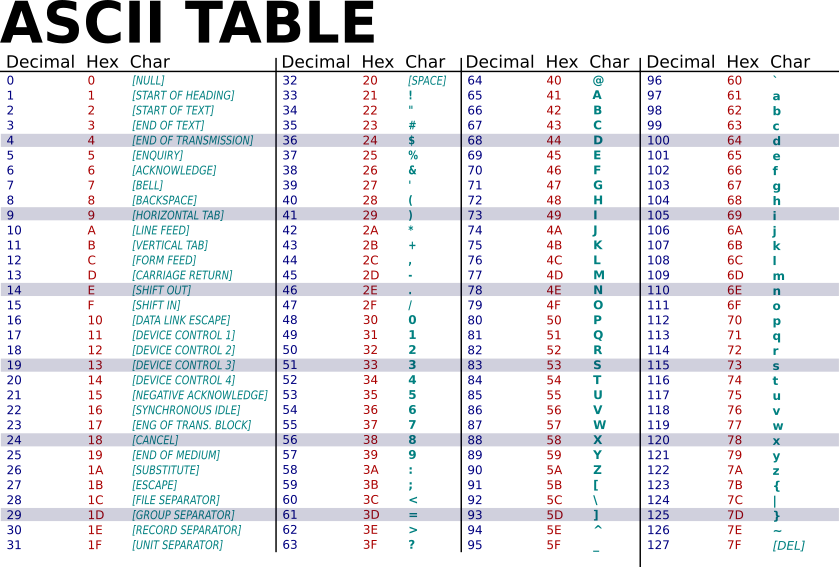
\includegraphics[width=\linewidth]{./gfx/ASCII_table}\newline
	\tiny ASCII: American Standard Code for Information Interchange\newline
	Quelle: \url{source: https://commons.wikimedia.org/wiki/File:ASCII-Table-wide.svg}
\end{columns}
%
\end{frame}

% =========================================================================== %

\begin{frame}{Datentypen}
%
\begin{itemize}
\item Jedem Ausdruck (\zB jeder Variable) zugeordnete Information: Was ist das?
\item Gibt Kontext für Rechnungen vor.
\item Beispiel: Text vs. Zahl:
	\begin{itemize}
	\item \inPy{"1" + "2"} \thus~ \inPy{"12"}
	\item \inPy{1 + 2} \thus~ \inPy{3}
	\end{itemize}
\item Datentypen:
	\begin{itemize}
	\item \inPy{int} -- Ganzzahlen
	\item \inPy{float} -- Reelle Kommazahlen
	\item \inPy{complex} -- Komplexe Kommazahlen: \inPy{z = 5.3 - 1j}
	\item \inPy{str} -- Text (\enquote{String})
	\end{itemize}
\item Datentyp herausfinden: \inPy{print(type(Ausdruck))}
\end{itemize}
%
\end{frame}

% =========================================================================== %

\begin{frame}[fragile]{Kommentare}
%
\begin{minipage}[t]{.44\linewidth}
\begin{itemize}
\item Text-Teile, die vom Interpreter ignoriert werden
\item Erinnerungen und Erklärungen für uns als ProgrammiererInnen
\item Zeilen zum Testen schnell ein- und ausschalten
\item Beginnen mit Raute (\texttt{\#})
\item Gehen bis zum Ende der Zeile
\end{itemize}
\end{minipage}
%
\begin{minipage}[t]{.55\linewidth}
\phantom{x}
\begin{codebox}[Code mit Kommentaren]
\begin{minted}[linenos, fontsize=\scriptsize]{python}
print("Hello World")  # Textausgabe

# Auch als eigene Zeile

# Verschachtelte # Kommentare existieren nicht

# print("Code, der nicht ausgeführt wird")
\end{minted}
\end{codebox}
\end{minipage}
%
\end{frame}

\end{document}

% MAREI!!
% whom do I give credit? Where?